\documentclass[nooutcomes]{ximera}
%% handout
%% space
%% newpage
%% numbers
%% nooutcomes


\newcommand{\RR}{\mathbb R}
\renewcommand{\d}{\,d}
\newcommand{\dd}[2][]{\frac{d #1}{d #2}}
\renewcommand{\l}{\ell}
\newcommand{\ddx}{\frac{d}{dx}}
\newcommand{\dfn}{\textbf}
\newcommand{\eval}[1]{\bigg[ #1 \bigg]}

\usepackage{multicol}

\renewenvironment{freeResponse}{
\ifhandout\setbox0\vbox\bgroup\else
\begin{trivlist}\item[\hskip \labelsep\bfseries Solution:\hspace{2ex}]
\fi}
{\ifhandout\egroup\else
\end{trivlist}
\fi} %% we can turn off input when making a master document
\usepackage{fullpage}

\title{3.5 Derivatives of Trig Functions}  

\begin{document}
\begin{abstract}		\end{abstract}
\maketitle


%problem1
\begin{problem} \hfil
	\begin{enumerate}
	\item Suppose we're given the right triangle below.  Express $\sin(\theta)$ and $\cos(\theta)$ in terms of the sides of the triangle.

	\begin{image}
	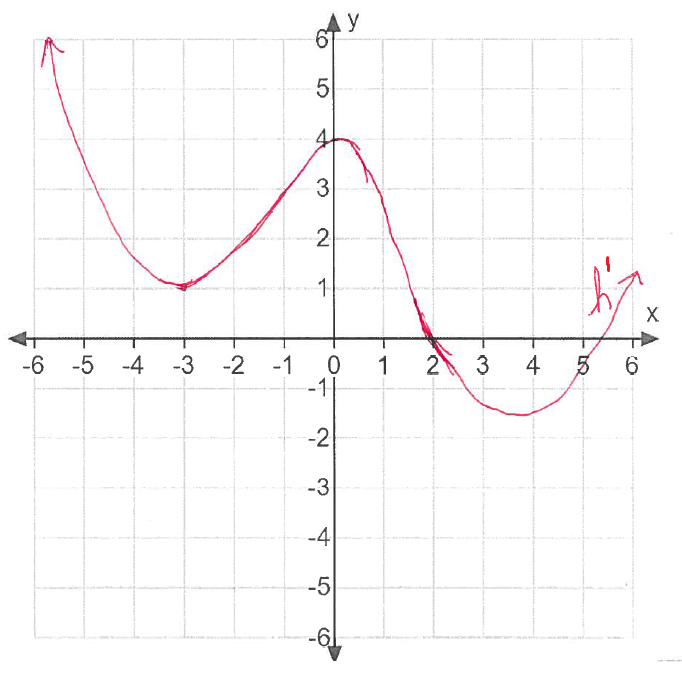
\includegraphics[scale=.3]{figure1.png}
	\end{image}
	\begin{freeResponse}
	$\sin(\theta)=\frac{B}{C}=B$ and $\cos(\theta)=\frac{A}{C}=A$ 
	\end{freeResponse}

	\item Suppose we are given the triangle below.  
		\begin{image}
		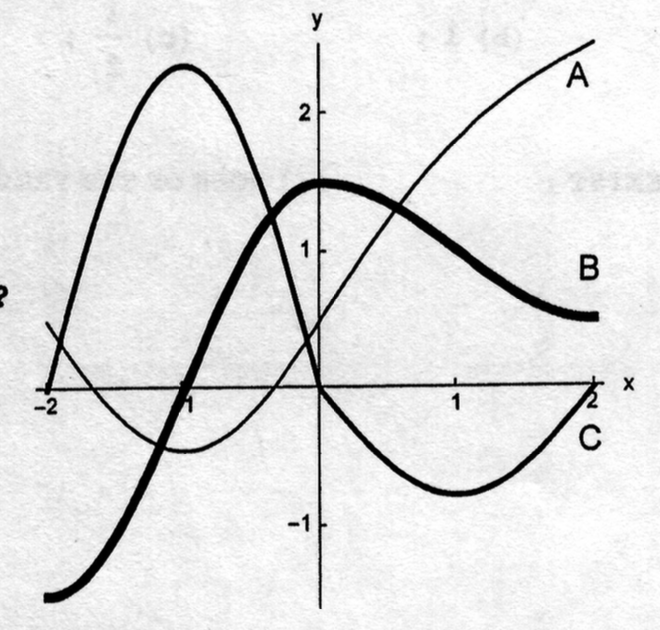
\includegraphics[scale=.3]{figure2.png}
		\end{image}

		\begin{enumerate}
	\item Find the length of the sides A and B.
	\begin{freeResponse}
	This is an isosceles triangle. $A=B$  Using the Pythagorean Theorem:
	\begin{align*}
	A^2+B^2&=1^2\\
	2A^2&=1 \\ 	
	A^2&=\frac{1}{2}\\
	A&=\sqrt{\frac{1}{2}}=\frac{\sqrt{2}}{2}\\
	B&=\sqrt{\frac{1}{2}}=\frac{\sqrt{2}}{2}
	\end{align*}
	\end{freeResponse}

	\item Express $\sin\left(\frac{\pi}{4}\right)$ and $\cos\left(\frac{\pi}{4}\right)$ in terms of the sides of the triangle.

	\begin{freeResponse}
	$\sin\left(\frac{\pi}{4}\right)=\frac{B}{C}=\frac{\sqrt{2}}{2}$ and $\cos\left(\frac{\pi}{4}\right)=\frac{A}{C}=\frac{\sqrt{2}}{2}$

	\end{freeResponse}
	\end{enumerate}

	\item Suppose we are given the triangle below.  
		\begin{image}
		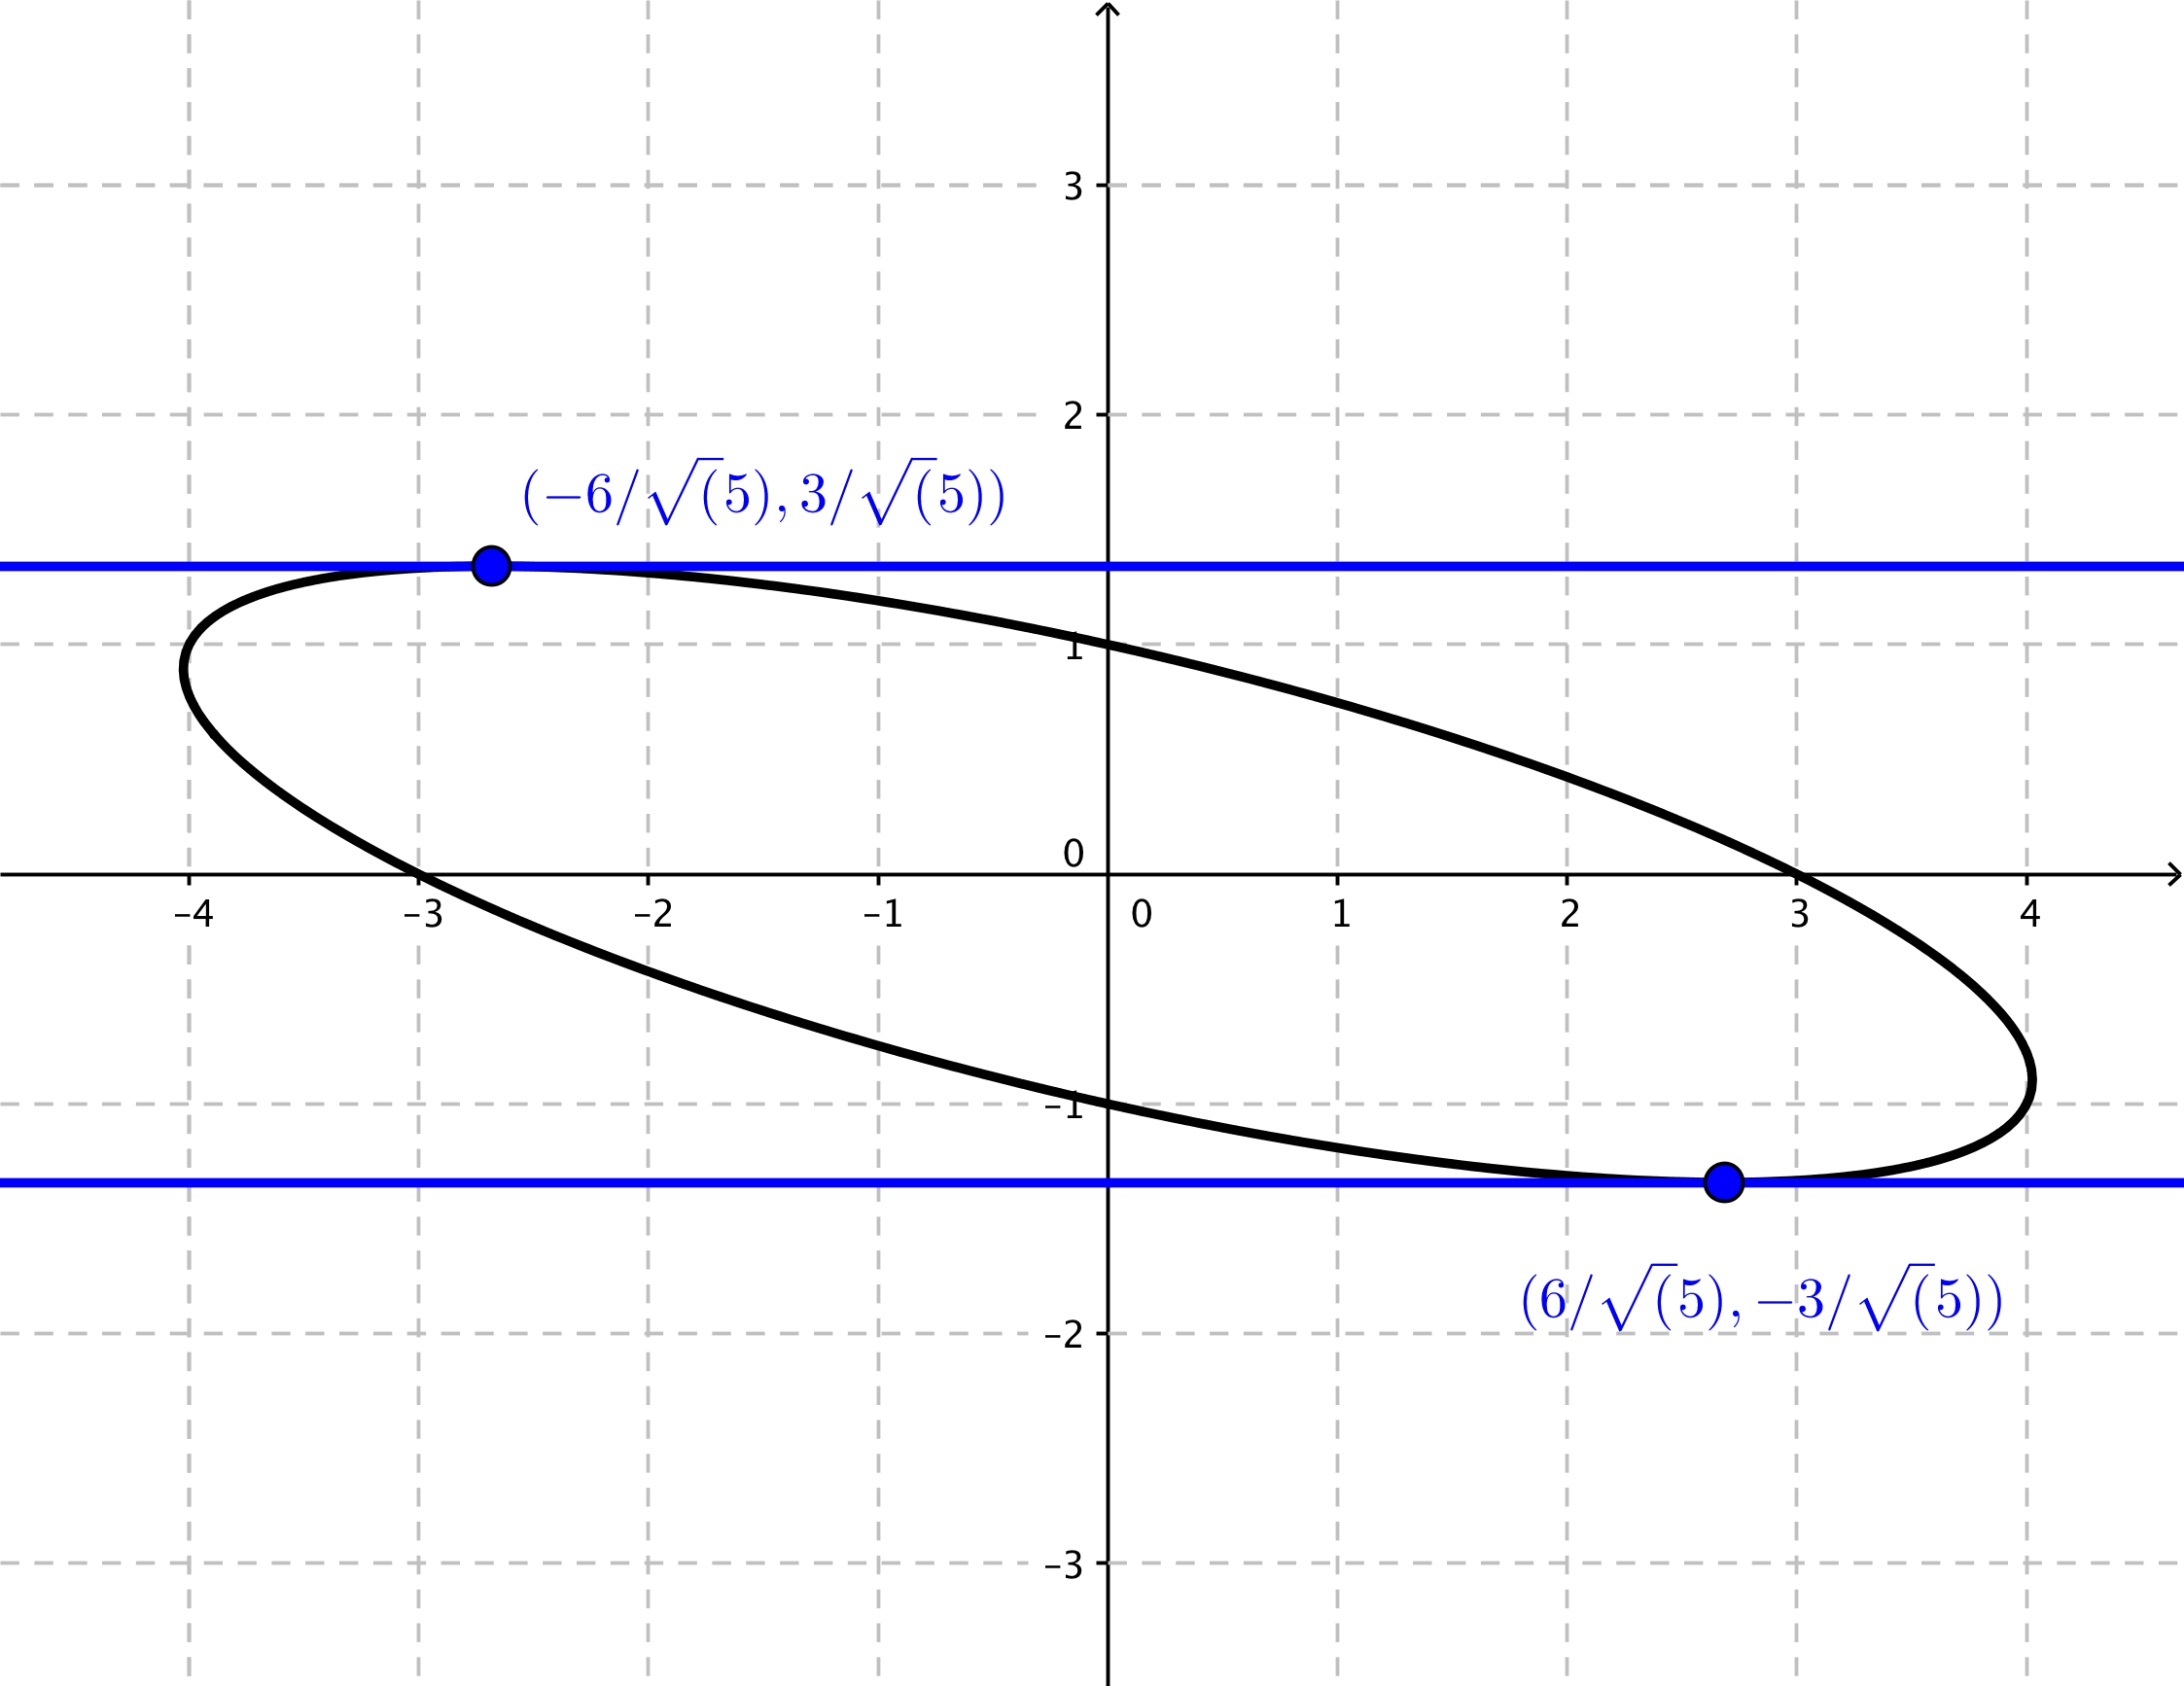
\includegraphics[scale=.5]{figure3.png}
		\end{image}

		\begin{enumerate}
	\item Find the length of the sides A and B.
	\begin{freeResponse}
	You might remember this as a 30/60/90 triangle.  To find the lengths of the sides of the triangle, we create a triangle as in the figure below.  All the angles in this triangle are of 60 degrees, therefore, this is an equilateral triangle 
		\begin{image}
		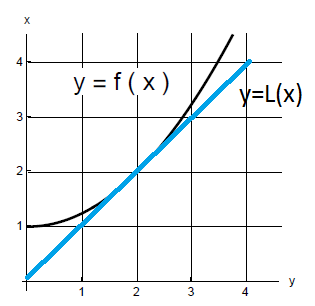
\includegraphics[scale=.5]{figure4.png}
		\end{image}
	Now that we have an equilateral triangle, we have $C=C=2A$.  Thus, $1=2A \implies A=\frac{1}{2}$ \\
	To find B, we use the Pythagorean Theorem.
	\begin{align*}
	\left(\frac{1}{2}\right)^2+B^2&=1^2\\
	\frac{1}{4}+B^2&=1 \\ 	
	B^2&=\frac{3}{4}\\
	B&=\sqrt{\frac{3}{4}}=\frac{\sqrt{3}}{2}
	\end{align*}
	\end{freeResponse}

	\item Express $\sin\left(\frac{\pi}{3}\right)$ and $\cos\left(\frac{\pi}{3}\right)$ in terms of the sides of the triangle.

	\begin{freeResponse}
	$\sin\left(\frac{\pi}{3}\right)=\frac{\sqrt{3}}{2}$ and $\cos\left(\frac{\pi}{3}\right)=\frac{1}{2}$

	\end{freeResponse}
	\end{enumerate}

\item Suppose we are given the triangle below.  
		\begin{image}
		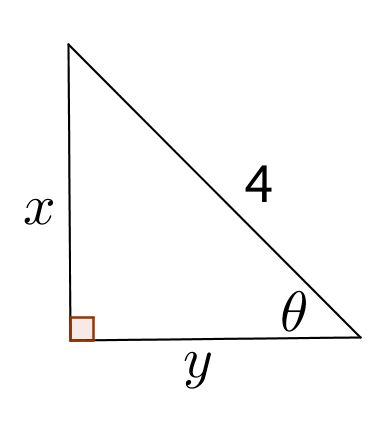
\includegraphics[scale=.5]{figure5.png}
		\end{image}

		\begin{enumerate}
	\item Find the length of the sides A and B.
	\begin{freeResponse}
	We've actually already found the lengths of the sides for this type of triangle in part c.  $B=\sqrt{\frac{3}{4}}=\frac{\sqrt{3}}{2}$ and $A=\frac{1}{2}$ 
	\end{freeResponse}

	\item Write $\sin\left(\frac{\pi}{6}\right)$ and $\cos\left(\frac{\pi}{6}\right)$ in terms of the sides of the triangle.

	\begin{freeResponse}
	$\sin\left(\frac{\pi}{6}\right)=\frac{A}{C}=\frac{1}{2}$ and $\cos\left(\frac{\pi}{6}\right)=\frac{B}{C}=\frac{\sqrt{3}}{2}$

	\end{freeResponse}
	\end{enumerate}



	\item 
For any point P(x,y) on the unit circle, we can express its coordinates in terms of $\sin(\theta)$ and $\cos(\theta)$.
Here $\theta$ is the radian measure of the angle in standard position whose terminal side is the line through the origin and the point $P(x,y)$.
\begin{image}
		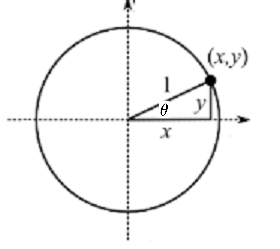
\includegraphics[scale=.8]{figure12.png}
		\end{image}
		\begin{freeResponse}
	$(x,y)=(\cos(\theta),\sin(\theta))$
	\end{freeResponse}

	\item  Use all of the above information to label the given points on the unit circle.
		\begin{image}
		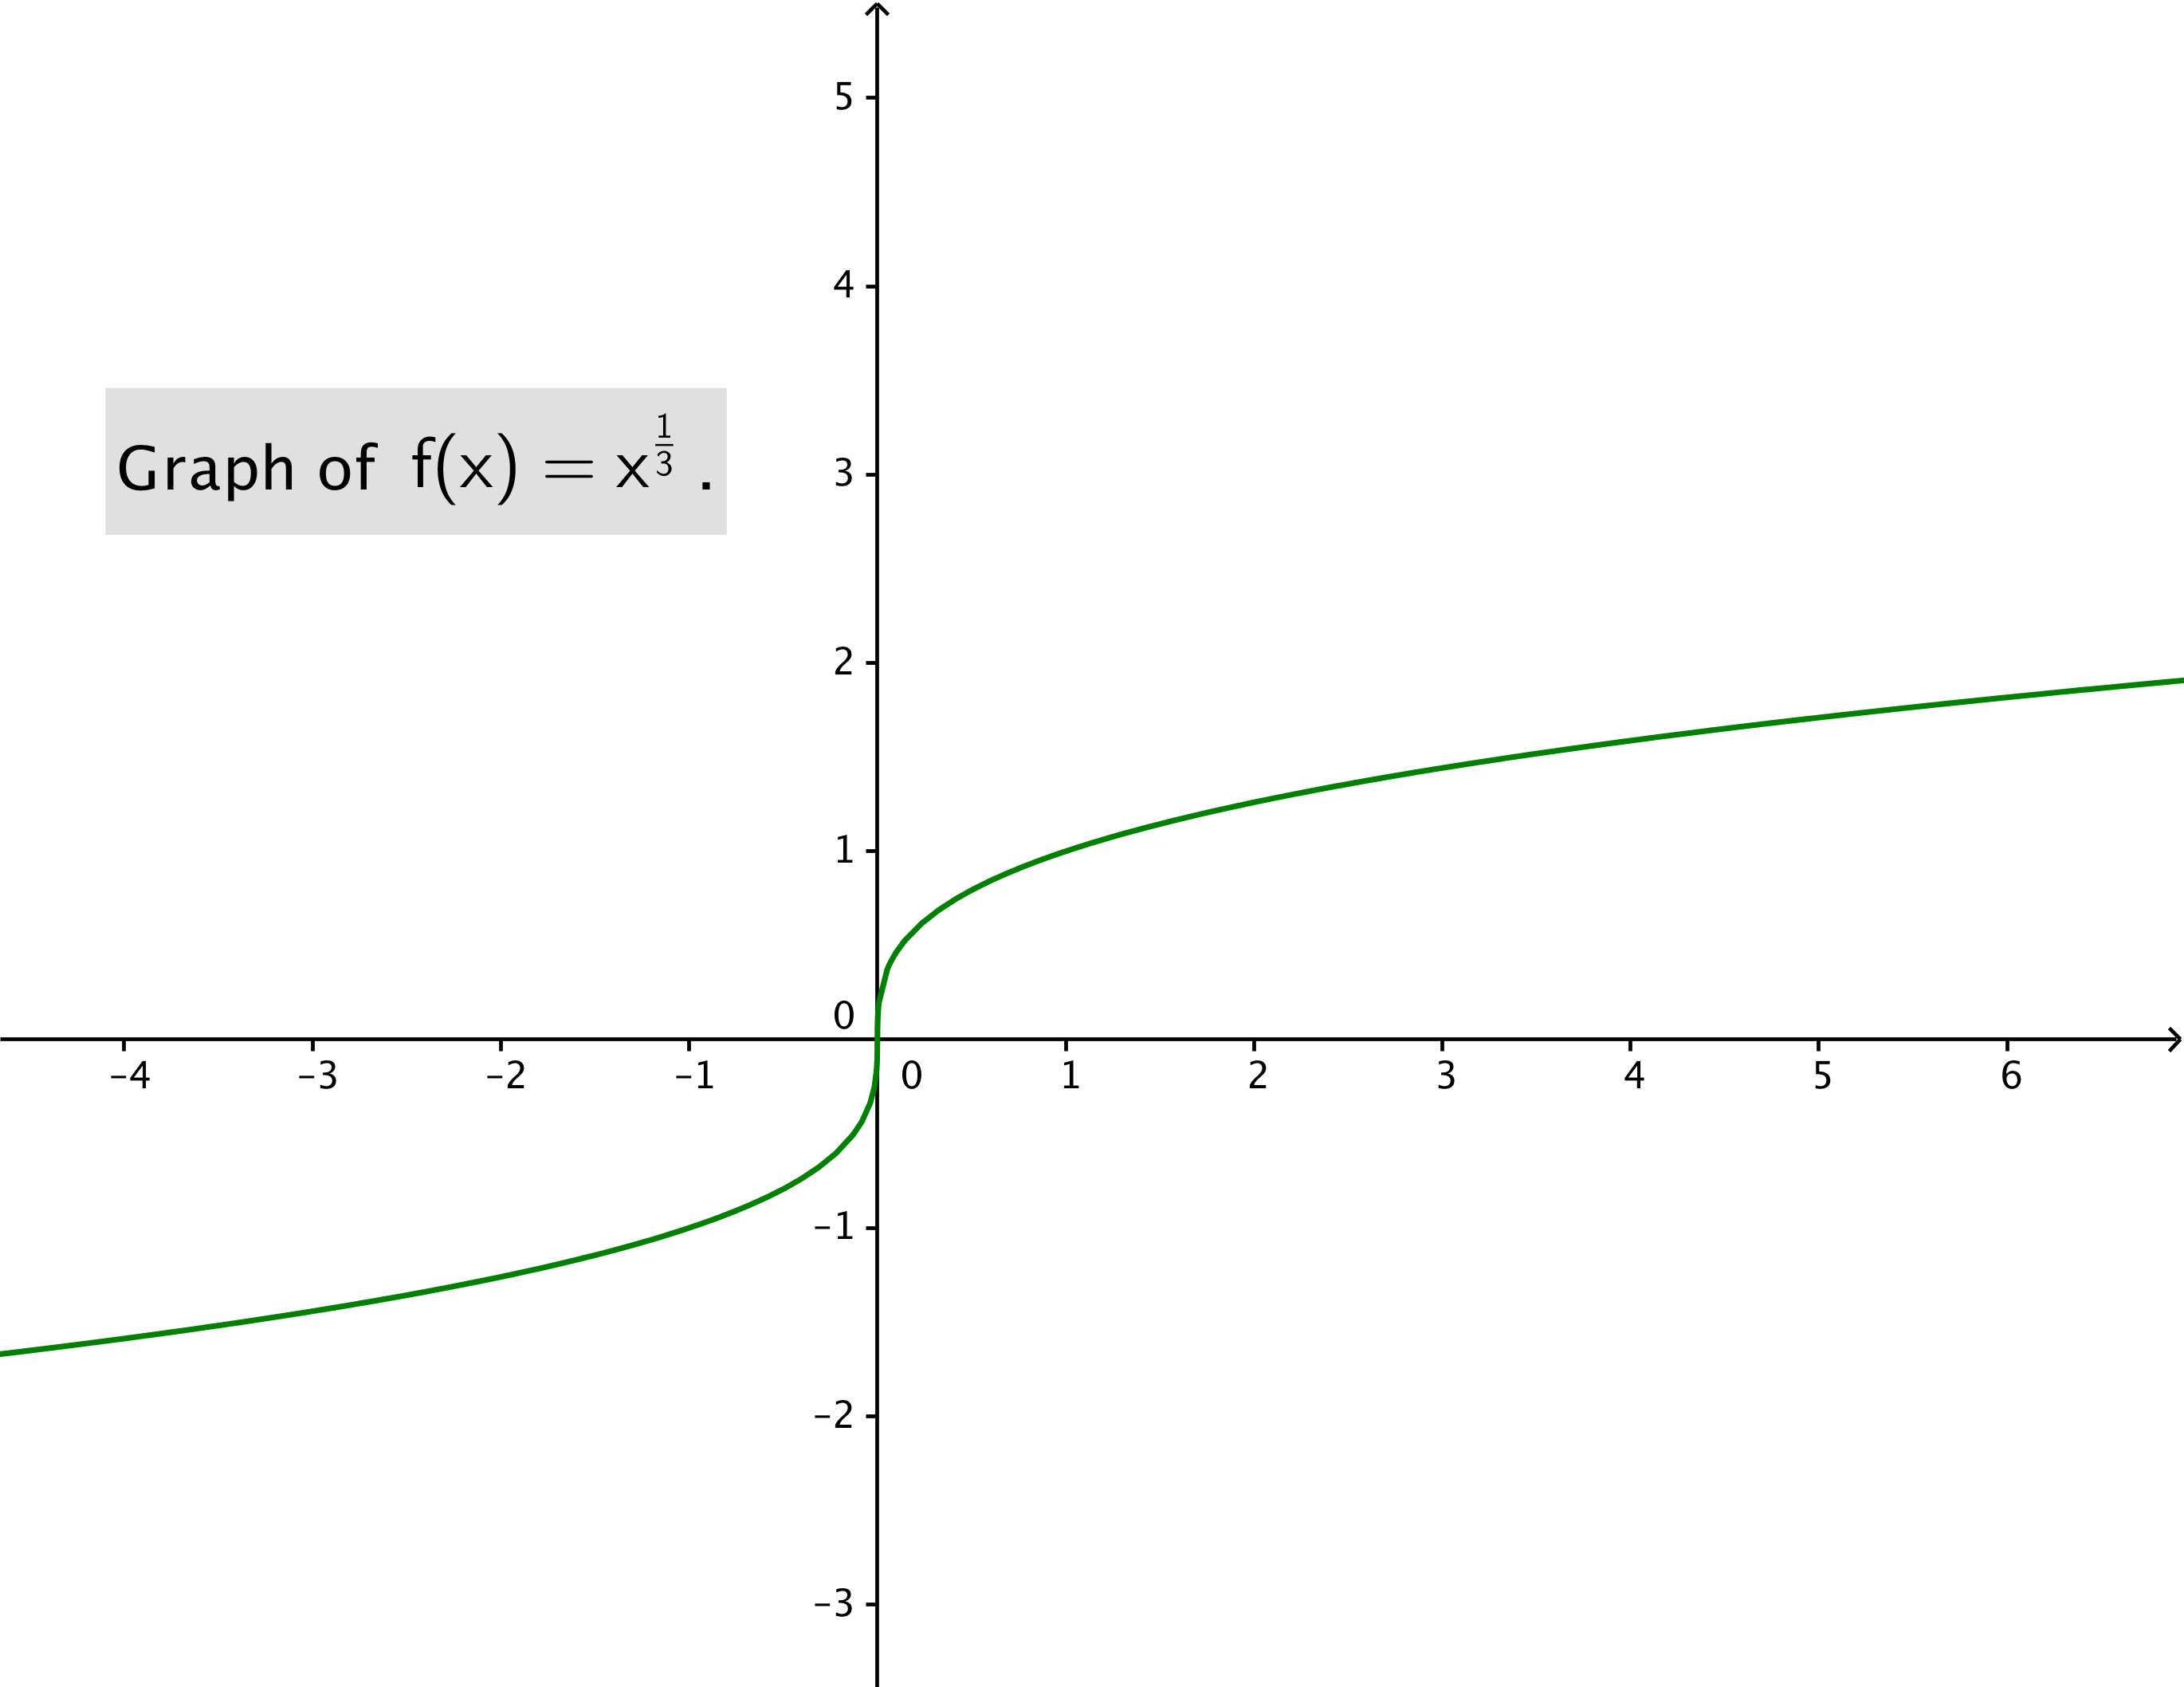
\includegraphics{figure6.png}
		\end{image}

		\begin{freeResponse} \hfil
		\begin{image}
		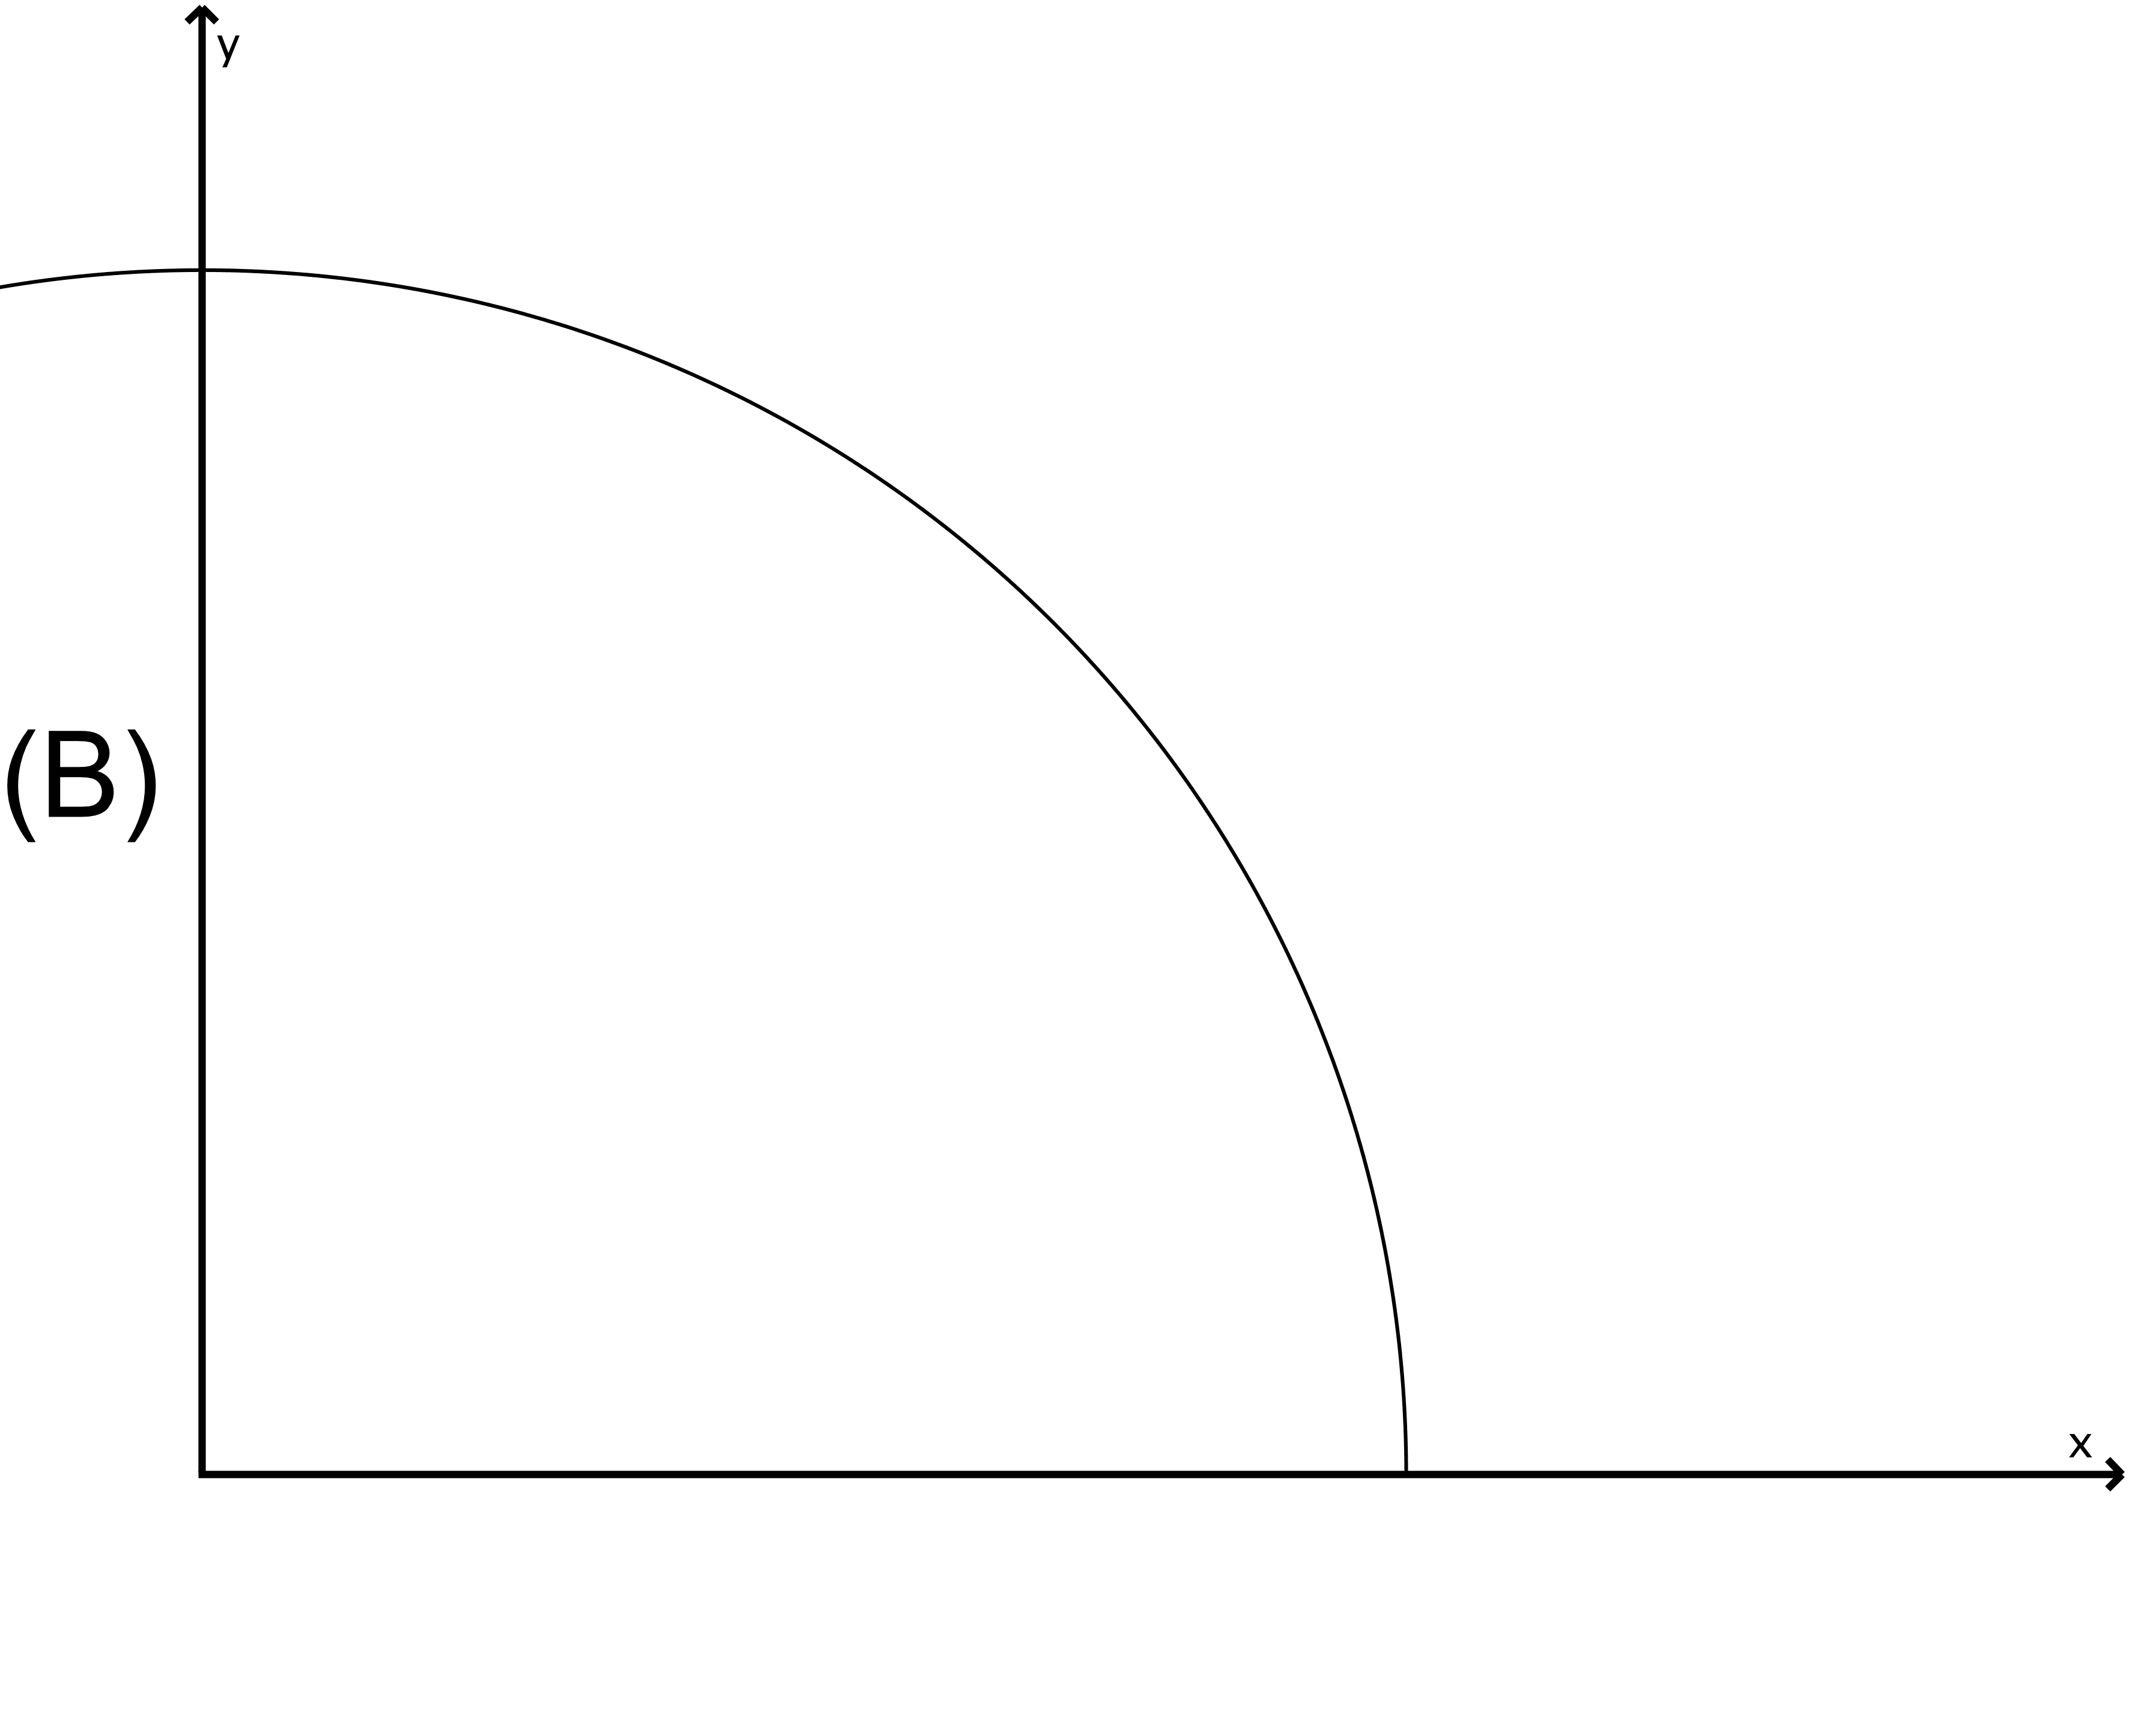
\includegraphics[scale=.6]{figure7.png}
		\end{image}
		\end{freeResponse}
	\end{enumerate}

\end{problem}


%problem2
\begin{problem}

  Find all real numbers which satisfy each of the equations.  In the previous problem, we used $\theta$ to denote the radian measure of the angle.  However, we can use any variable to represent the angle measure.  For example, in part a, $x$ is the variable representing the radian measure of the angle.
  \begin{enumerate}
    \item
      $\cos(x) = 1$
      \begin{freeResponse}
        This is asking for the collection of all angles such that cosine of that angle equals 1.

        The unit circle shows that one such angle is $0$ (since $\cos(0) = 1$).
        There is a slight trick here: since cosine has period $2\pi$ we actually have $\cos(0 + 2\pi n) = 1$ for every integer $n$.
        In summary, $x = 2\pi n$, where $n$ is any integer, gives all the solutions to this equation.
      \end{freeResponse}

    \item
      $\sin(3 \theta) = \sqrt{3}/2$ for $0 \leq \theta \leq 2\pi$
      \begin{freeResponse}
        Finding all numbers $\theta$ with $0 \leq \theta \leq 2\pi$ that satisfy $\sin(3 \theta) = \sqrt{3}/2$ is a bit tricky.
        We first perform a useful trick from algebra~---~variable substitution.

        Let $x = 3\theta$.
        So, we are trying to find all numbers $x$ such that $\sin(x) = \sqrt{3}/2$ for $0 \leq x/3 \leq 2\pi$.
        Then $ x= \frac{\pi}{3} + 2 \pi n$ or $ x = \frac{2 \pi }{3} + 2 \pi n $ for $n$ any integer as long as $0 \leq \theta \leq 2\pi$
        Since $x = 3 \theta$, we can solve for $\theta$ to obtain $\theta = \pi/9 + (2 \pi n)/3$ or $\theta = (2\pi)/9 + (2\pi n)/3$, where $n$ is again any integer as long as $0 \leq \theta \leq 2\pi$.
        We are only looking for solutions of $\theta$ in $[0, 2\pi ]$, and so our solutions are
        \[
        \theta = \frac{\pi}{9}, \frac{2\pi}{9}, \frac{7\pi}{9}, \frac{8\pi}{9}, \frac{13\pi}{9}, \frac{14\pi}{9}. 
        \]
      \end{freeResponse}
  \end{enumerate}
\end{problem}


%problem3
\begin{problem} \hfil

\begin{enumerate}
	\item Graph $f(\theta)=\sin(\theta)$ and $g(\theta)=\cos(\theta)$ from $[-\frac{\pi}{8},2\pi+\frac{\pi}{8}]$
		\begin{freeResponse} \hfil
		\begin{image}
		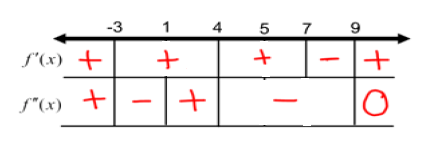
\includegraphics[scale=.3]{figure8.png}
		\end{image}
		\begin{image}
		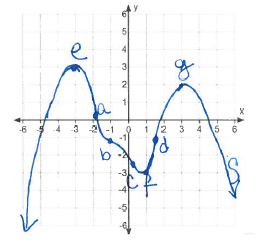
\includegraphics[scale=.3]{figure9.png}
		\end{image}
		\end{freeResponse}

	\item For $0 \leq \theta \leq 2\pi$, find the following values or intervals.
		\begin{enumerate}
			\item Where does $f'(\theta)=0$?
		\begin{freeResponse}
			$f'(\theta)=0$ at $\theta=\frac{\pi}{2},\frac{3\pi}{2}$
		\end{freeResponse}
			\item Where is $f'$ negative?  Where is it positive?
		\begin{freeResponse}
			$f'$ is negative on $\left( \frac{\pi}{2},\frac{3 \pi}{2}\right)$.  $f'$ is positive on $ \left( 0,\frac{\pi}{2} \right)$ , $ \left( \frac{3 \pi}{2},2 \pi \right)$
		\end{freeResponse}
			\item Where is $f'$:
			\begin{enumerate}
			\item negative and increasing?
				\begin{freeResponse}
					$(\pi,\frac{3\pi}{2})$
				\end{freeResponse}
			\item negative and decreasing?
				\begin{freeResponse}
					$(\frac{\pi}{2},\pi)$
				\end{freeResponse}
			\item positive and increasing?
				\begin{freeResponse}
					$(\frac{3\pi}{2},2\pi)$
				\end{freeResponse}
			\item positive and decreasing?
				\begin{freeResponse}
					$(0,\frac{\pi}{2})$
				\end{freeResponse}
			\end{enumerate}
			\item Where does $g'(\theta)=0$?
		\begin{freeResponse}
			$g'(\theta=0$ at $\theta=0,\pi,2\pi$
		\end{freeResponse}
			\item Where is $g'$ negative?  Where is it positive?
		\begin{freeResponse}
			$g'$ is negative on $(0,\pi)$ and positive on $(\pi,2\pi)$
		\end{freeResponse}
			\item Where is $g'$:
			\begin{enumerate}
			\item negative and increasing?
				\begin{freeResponse}
					$(\frac{\pi}{2},\pi)$
				\end{freeResponse}
			\item negative and decreasing?
				\begin{freeResponse}
					$(0,\frac{\pi}{2})$
				\end{freeResponse}
			\item positive and increasing?
				\begin{freeResponse}
					$(\pi,\frac{3\pi}{2})$
				\end{freeResponse}
			\item positive and decreasing?
				\begin{freeResponse}
					$(\frac{3\pi}{2},2\pi)$
				\end{freeResponse}
			\end{enumerate}
		\begin{freeResponse}
			$g'$ is steepest at $\frac{\pi}{2},\frac{3\pi}{2}$
		\end{freeResponse}
		\end{enumerate}
	\item Use the above information to sketch a graph of $f'$ and $g'$.
		\begin{freeResponse} \hfil
		\begin{image}
		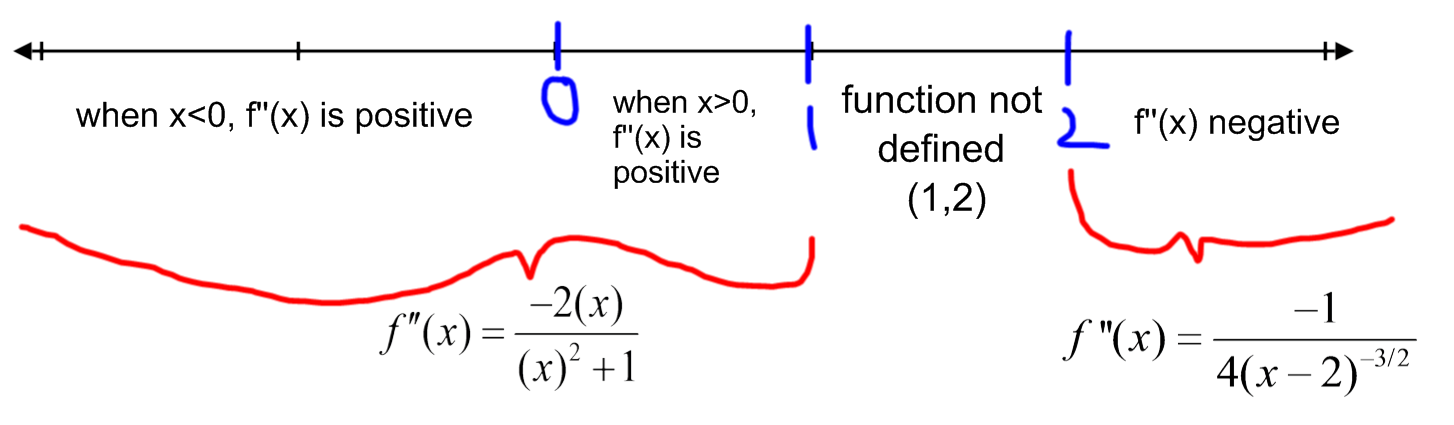
\includegraphics[scale=.3]{figure10.png}
		\end{image}
		\begin{image}
		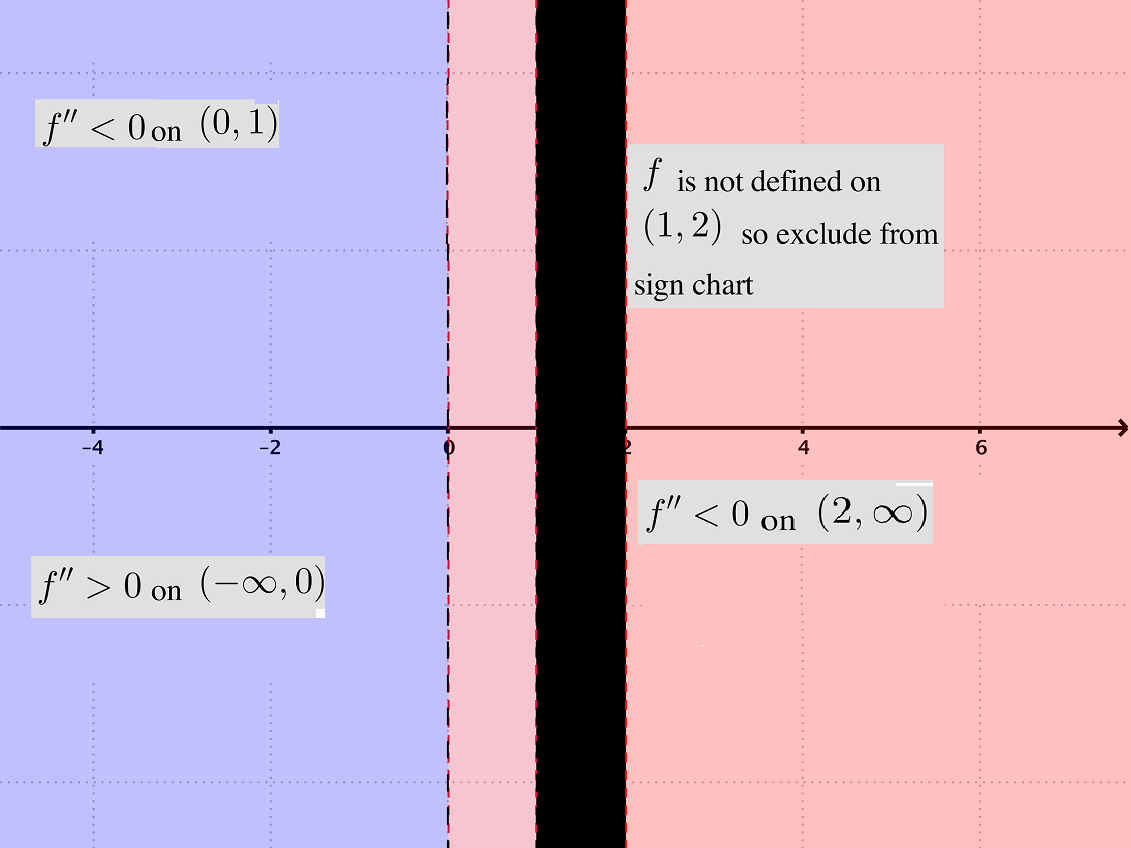
\includegraphics[scale=.3]{figure11.png}
		\end{image}
		\end{freeResponse}

	\item Based on the graphs of $f'$ and $g'$, what might the equation for $f'$ and $g'$ be?
		\begin{freeResponse}
			It appears $f'(\theta)=\cos(\theta)$ and $g'(\theta)=-\sin(\theta)$
		\end{freeResponse}


\end{enumerate}
\end{problem}


%problem 4
\begin{problem}
Find the following limits:

	\begin{enumerate}
	
	\item  $\lim_{x \to 0} \frac{\sin(8x)}{x}$
			\begin{freeResponse}
			\begin{align*}
			\lim_{x \to 0} \frac{\sin(8x)}{x} &= \lim_{x \to 0} \frac{\sin(8x)}{x} \cdot \frac{8}{8}  \\
			&= 8 \lim_{x \to 0} \frac{\sin(8x)}{8x}  \\
			&= 8 \lim_{u \to 0} \frac{\sin(u)}{u}  \\
			&= 8 \cdot 1 = 8
			\end{align*}
			where $u = 8x$.  
			\end{freeResponse}
			
	
	\item  $\lim_{x \to 0} \frac{x}{\tan(5x)}$
			\begin{freeResponse}
			\begin{align*}
			\lim_{x \to 0} \frac{x}{\tan(5x)} &= \lim_{x \to 0} \frac{x}{\frac{\sin(5x)}{\cos(5x)}}  \\
			&= \lim_{x \to 0} \left( \frac{x}{1} \cdot \frac{\cos(5x)}{\sin(5x)} \right)  \\
			&= \lim_{x \to 0} \left( \cos(5x) \frac{x}{\sin(5x)} \cdot \frac{5}{5} \right)  \\
			&= \frac{1}{5} \left( \lim_{x \to 0} \cos(5x) \right) \left( \lim_{x \to 0} \frac{5x}{\sin(5x)} \right)  \\
			&= \frac{1}{5} (1) (1) = \frac{1}{5}
			\end{align*}
			\end{freeResponse}
			
			
			
	\end{enumerate}
\end{problem}
	
%problem 5		
\begin{problem}
Find the derivative of the following functions:

	\begin{enumerate}
	
	%part a
	\item  $f(x) = \frac{x+5}{7x^6 + \cot(x)}$
			\begin{freeResponse}
			\begin{align*}
			f'(x) &= \frac{(7x^6 + \cot(x))(1) - (x+5)(42x^5 - \csc^2(x))}{(7x^6 + \cot(x))^2}  \\
			&= \frac{7x^6 + \cot(x) - (x+5)(42x^5 - \csc^2(x))}{(7x^6 + \cot(x))^2}.
			\end{align*}
			\end{freeResponse}
			
			
			
	%part b
	\item  $f(x) = \sin(x) \cos(x)$
			\begin{freeResponse}
			$$f'(x) = (\cos(x))(\cos(x)) + (\sin(x))(-\sin(x)) = \cos^2(x) - \sin^2(x).$$
			\end{freeResponse}
			
			
			
	%part c
	\item  $f(x) = \frac{e^x \tan(x)}{\sec(x) + 2}$
			\begin{freeResponse}
			\begin{align*}
			f'(x) &= \frac{(\sec(x)+2)(e^x \tan(x) + e^x \sec^2(x)) - e^x \tan(x) (\sec(x) \tan(x))}{(\sec(x) + 2)^2}  \\
			&= \frac{e^x[(\sec(x) + 2)(\tan(x) + \sec^2(x)) - \sec(x) \tan^2(x)]}{(\sec(x) + 2)^2}.
			\end{align*}
			\end{freeResponse}
			
			
			
	%part d
	\item  $f(x) = \sin(x) \cos(x) e^{3x}$
			\begin{freeResponse}
			\begin{align*}
			f'(x) &= \ddx[\sin(x) \cos(x)] e^{3x} + (\sin(x) \cos(x)) \ddx(e^{3x})  \\
			&= (\cos^2(x) - \sin^2(x))e^{3x} + 3e^{3x} \sin(x) \cos(x)  \\
			&= e^{3x}(\cos^2(x) + 3\sin(x) \cos(x) - \sin^2(x)).
			\end{align*}
			\end{freeResponse}
			
			
			
	\end{enumerate}
		
\end{problem}	

%problem 6
\begin{problem}
Let $f(x) = \sin(x)$ and $g(x) = \cos(x)$.  Can you compute $f^{(48)}(x)$, $g^{(42)}(x)$, and $g^{(39)}(x)$ ?  

\begin{freeResponse}
Let's find the first several derivatives of $f(x)=sin(x)$.

	\begin{align*}
	f^{(0)}(x)&=\sin(x)\\
	f^{(1)}(x)&=\cos(x)\\
	f^{(2)}(x)&=-\sin(x)\\
	f^{(3)}(x)&=-\cos(x)\\
	f^{(4)}(x)&=\sin(x)
	\end{align*}

  Recall that, for $n$ a nonnegative integer,
  $$f^{(4n)}(x) = f(x) = \sin(x) \quad \text{and} \quad g^{(4n)}(x) = g(x) = \cos(x).$$
  Thus: \\ 
  $f^{(48)}(x) =f(x)= \sin(x)$ \\
 $g^{(42)}(x) =g^{(40+2)}(x)= g^{(2)}(x) = g''(x) = - \cos(x)$  \\
$g^{(39)}(x) =g^{(36+3)}(x)= g^{(3)}(x) = g'''(x) = \sin(x)$  



\end{freeResponse}

\end{problem}
	



	
	
			



		
%problem7

\begin{problem} \hfil

\begin{enumerate}
	\item Let $f(x)= \frac{x^2-5x}{(x+5)\sin(x)}$.  Compute $f'(x)$

	\begin{freeResponse}	
	$f'(x)= \frac{(2x-5)(x+5)\sin(x)-(x^2-5x)(\sin(x)+(x+5)\cos(x))}{(x+5)^2 \cdot\sin^2(x)}$

	\end{freeResponse}

	\item Evaluate the limit. $\lim_{x \to 5} \frac{x^2-5x}{\sin(x-5)}$

	\begin{freeResponse}
	\begin{align*}
	\lim_{x \to 5} \frac{x^2-5x}{\sin(x-5)}=\lim_{x \to 5} \frac{x(x-5)}{\sin(x-5)}\\
	&=\lim_{x \to 5}(x) \cdot  \lim_{x \to 5}\frac{x-5}{\sin(x-5)}\\\\
	&=\lim_{x \to 5}(x) \cdot  \lim_{x \to 5}\frac{1}{\frac{\sin(x-5)}{x-5}}\\\\
	&=\lim_{x \to 5}(x) \cdot \frac{1}{ \lim_{x \to 5}\frac{\sin(x-5)}{x-5}}\\\\
	& \text{if we let}\ u=x-5\ \text{we have:}\\
	&=\lim_{x \to 5}(x) \cdot  \frac{1}{\lim_{u \to 0}\frac{\sin(u)}{u}}\\\\
	&= 5(1)=5
	\end{align*}
	\end{freeResponse}

\end{enumerate}
\end{problem}		
		
%problem8		
\begin{problem}
Find values for $a$, $b$, and $c$ so that the following function is both continuous and differentiable everywhere.

$f(x) =   \left\{ \begin{array}{cl}
	a \sin(x) + b \cos(x)		 	&	\qquad \text{if } x < 0					\\
	ax^2 + bx + c   				&	\qquad \text{if } x \geq 0	 \end{array} \right.  $
		\begin{freeResponse}
		The function $f$ is differentiable for $x<0$ since $f$ is a combination of trigonometric functions.  $f$ is also differentiable $x>0$ since $f$ is a polynomial.  We need to focus on $x=0$.  Since $f$ is differentiable everywhere, $f$ must also be differentiable at $x=0$ and therefore continuous at $x=0$.  Therefore: \\\\
We need that $\lim_{x \to 0^-} f(x) = \lim_{x \to 0^+} f(x)$ and $\lim_{x \to 0} f(x)=f(0)$.  Observe that
		
		\begin{itemize}
		
		\item $\lim_{x \to 0^-} f(x) 
		= \lim_{x \to 0^-} (a\sin(x) + b\cos(x))
		= b(1) = b$.
		
		\item  $ \lim_{x \to 0^+} f(x)
		= \lim_{x \to 0^+} ax^2 + bx + c 
		= c$.
		
		\end{itemize}
		
		Thus, we must have that $b = c$\\\\
		Next, if $f'(0)$ exists, then:
		\begin{align*}
		f'(0)&=\lim_{x\to 0} \frac{f(x)-f(0)}{x-0}\\\\
		& \text{since}\ f(0)=a \cdot 0^2+b \cdot 0 +c =c\\\\
		& \lim_{x\to 0} \frac{f(x)-f(0)}{x-0}=\lim_{x\to 0} \frac{f(x)-c}{x}
		\end{align*}
		Since this limit exists, the left and right limits must be equal.
		
		\begin{align*}
		\lim_{x\to 0^+} \frac{f(x)-c}{x}&=\lim_{x\to 0^+} \frac{ax^2+bx+c-c}{x}\\
		&=\lim_{x\to 0^+} \frac{ax^2+bx}{x}\\
		&=\lim_{x\to 0^+} (ax+b)\\
		&=b
		\end{align*}
		\begin{align*}
		\lim_{x\to 0^-} \frac{f(x)-c}{x}&=\lim_{x\to 0^-} \frac{a \sin(x)+b \cos(x)-c}{x}\\
		&=\lim_{x\to 0^-} \frac{a \sin(x)}{x}+\lim_{x\to 0^-} \frac{b\cos(x)-c}{x}\\ \\
		& \text{we already found}\ b=c \ \text{so we have}\\
		&\lim_{x\to 0^-} \frac{a \sin(x)}{x}+\lim_{x\to 0^-} \frac{b \cos(x)-c}{x}=\lim_{x\to 0^-} \frac{a \sin(x)}{x}+\lim_{x\to 0^-} \frac{c\cdot \cos(x)-c}{x}\\
		&=a\cdot \lim_{x\to 0^-} \frac{ \sin(x)}{x}+c \cdot \lim_{x\to 0^-} \frac{\cos(x)-1}{x}\\ \\
		& \text{since}\ \lim_{x\to 0} \frac{\sin(x)}{x}=1 \text{and}\  \lim_{x\to 0} \frac{\cos(x)-1}{x}=0 \ \text{we have}\\
		&a\cdot \lim_{x\to 0^-} \frac{\sin(x)}{x}+c \cdot \lim_{x\to 0^-} \frac{\cos(x)-1}{x}=a
		\end{align*}

		This means in order for the derivative to exist, $a=b=c$.
		\end{freeResponse}
\end{problem}	














\end{document} 


















